\subsection{Y-Axis: Functional Decomposition}
\label{sec:y-axis}
The y-axis scaling focuses on the separation based on the responsibility for an
action which can be determined by the type of data or the type of work performed
for a transaction. While scaling on the x-axis could means ``everyone does
everything'', scaling on the y-axis specializes the workers splitting the whole
service in small services and assigning each service to a single worker. If we
combine the x-axis with the y-axis, we could have cluster of specialized workers
such that each cluster covers a different service, but workers in the same
cluster do the same job.

With regard to the data, differently from what happens in the x-axis, each
service should have its own non-shared data, thus segmenting it based on what
each service needs to have access to. This implies that the resources based on
the transactions demand for each service can be sized and optimized in order to
reduce the operational costs.

As for the x-axis, we provide an example of an architectural
approach which corresponds on the y-axis.

\subsubsection{An example: Microservice architecture}
Recalling the e-commerce example presented above, instead of replicating the
monolithic application and distribute the load equally between the clones, we
can identify logical components, that is different functional areas of the
application, such as account service, purchase service, product service.

\begin{figure}
	\begin{center}
		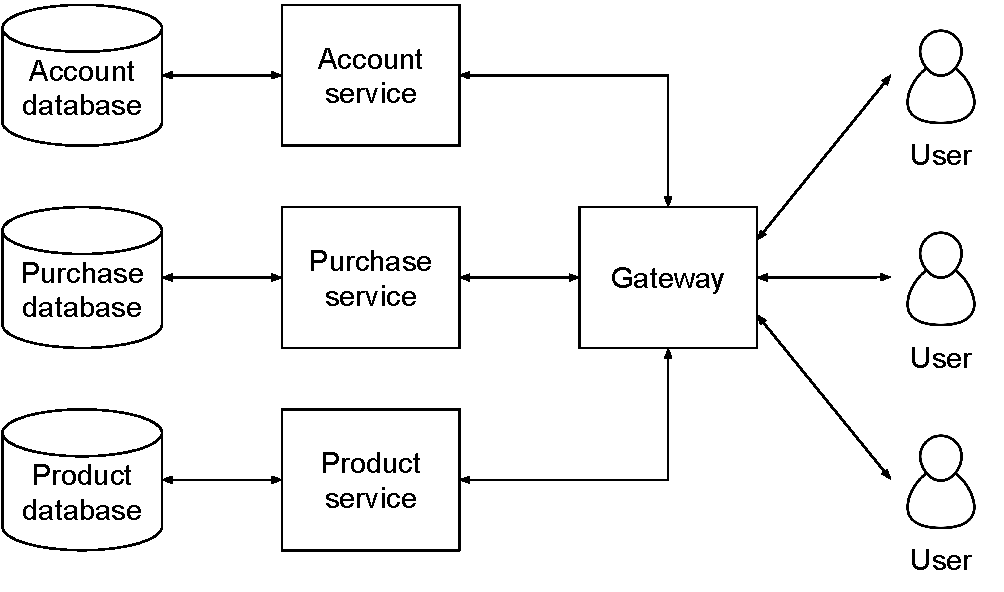
\includegraphics[width=.7\textwidth]{./res/img/microservice-architecture.pdf}
	\end{center}
	\caption{Example of a microservice architecture.}
	\label{fig:microservice-architecture}
\end{figure}

The diagram in \autoref{fig:microservice-architecture} summarises the
microservice architecture resulting from such division. The \emph{user} entity
condenses different client concepts (e.g. browser or mobile applications, bots,
humans, or others), while the \emph{gateway} represents what guides the requests
to the right service. In the case of a browser application, the gateway could
also exists only in it without needing a dedicated back end component, or it
could not exists at all, for example advertising the location of each service
and delegating to the users the responsibility to choose the right service. Each
service has its own non-shared database in order to be decoupled from other
services, which represents a good solution in the case of perfect isolated
services. More often, there could be some logical relations between data stored
in different services making necessary to implement a mechanism to maintain data
consistency. Such database separation opens the possibility to the services to
choose the database type which fits better for the service they are providing.
For example, the purchase service could use a SQL database taking advantage of
the different isolation levels to concurrently and consistently handle the
payments, while the product service could use a NoSQL database to tackle the
different properties of the products. The services could be organized around the
business capabilities (or ``something that a business does in order to generate
value'' \cite{bib:decompose-business-capability}), or decomposed by
responsibility for particular actions or for all the operations on entities of a
given type, but ideally each service should have only a small set of
responsibilities.

The main drawbacks of the Microservice Architecture Pattern
\cite{bib:microservice-architecture} are the increased complexity in development
and deployment. On the other hand, it has a number of advantages, among which:

\begin{itemize}
	\item \textbf{decoupling}. The functional decomposition of services
    decouples the components of the systems reflecting this behavior also in
    the database separation
	\item \textbf{fault isolation and design for failure}. Since the services
	implement different functionality of the system, they can be run on different
	processes leading to two consequences. The first one, as stated in
	\cite{bib:microservices-martin-fowler}, is that the application has to be
	designed thinking about a possible failure of a supplier, thus the client has
	to tolerate the failure of services responding as gracefully as possible. The
	second one is improved fault isolation, indeed, if a service has an unintended
	behavior, it is less likely to affect the other components of the system
	\item \textbf{scalability}. The services can be run on different more
	customized machines which better fit the resources requirements, hence making
	the vertical scaling more efficient wasting less resources. Moreover, if
	combined with the x-axis, it is possible to have a more fine-grained control
	on the horizontal scaling.
\end{itemize}

\subsubsection{Ethereum current state and proposals}
Currently Ethereum does not scale on this axis. A separation of responsibilities
based on the type of work can be identified looking at the node type. A miner is
responsible to collect pending transactions and build a valid block, while every
node is responsible to verify the blocks generated by the miners, but, as we
already discussed in \autoref{sec:x-axis-ethereum}, the transactions throughput
does not follow the trend of the number of miners.

Among the proposals from the Ethereum community to improve
scalability, no one takes evidently this direction. The different node roles,
although implementing different functions, do not define a functional
decomposition since they operate on the global shared data. This is the case of
Proof of Stake as well, which we briefly introduce in \autoref{sec:pos}, where
we can identify different node functions as we do in PoW.

\subsubsection{Proof of Stake}
\label{sec:pos}
Proof of Stake (PoS) is a class of algorithms through which a cryptocurrency
blockchain network achieves distributed consensus. As we have seen in
\autoref{sec:consensus:algorithm}, in PoW the truth is determined by heavy
computation done by the miners. In PoS, there are validators instead of miners
and the consensus depends on the \emph{stake} confirmed by each validator, which
consists in an economic deposit in the network's cryptocurrency (ether in this
case).

\begin{figure}
    \begin{center}
        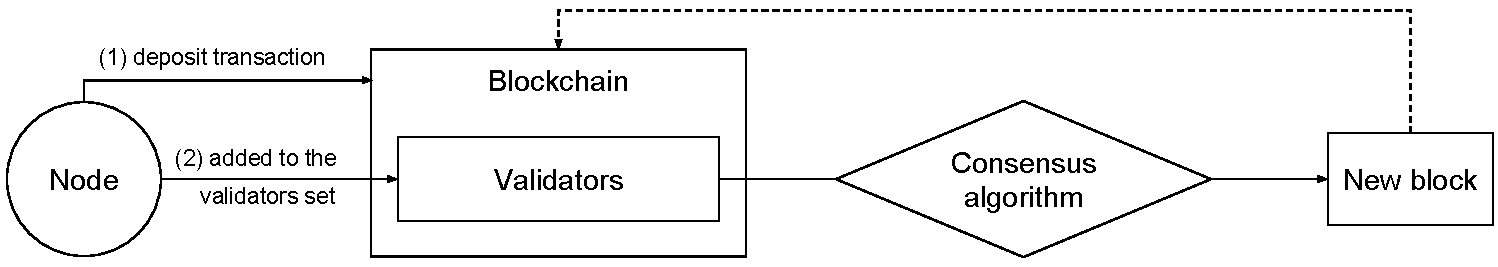
\includegraphics[width=\textwidth]{./res/img/pos.pdf}
    \end{center}
    \caption{Overview of a block creation in the Proof of Stake.}
    \label{fig:pos}
\end{figure}

\autoref{fig:pos} shows a creation of a new block at high level. If a node owns
an amount of the blockchain's base cryptocurrency, it can become a validator
sending a deposit transaction which locks a given value. Once the transaction
has successfully executed, the node becomes one of the validators. The consensus
algorithm determines how a validator is chosen in the set of validators to
\emph{propose} the next block, and then how the validators agree on which block
is canonical. Different type of PoS can be obtained by varying the consensus
algorithm and how the rewards are assigned.
